% CREATED BY DAVID FRISK, 2016
\chapter{Methodology}
Computational Fluid Dynamics (CFD) serves as a tool for studying fluid dynamics problems with high fidelity. The basic CFD workflow involves pre-processing, solving, and post-processing. In this chapter, we have outlined the CFD workflow that we followed to simulate the unsteady aerodynamics of fruit fly wing beat motion in STAR-CCM+. 
\\
\\
As mentioned in the introduction, we follow an approach to simulation where we consider the wing as rigid. In the pre-processing section preparation of geometry and computational domain, the dataset for simulating kinematics, and the generation of computational grid required for simulation are discussed. Further physics for the simulation is set up and solved with the aid of cluster computing platforms. In the final step of post-processing, results from the simulation are consolidated for analysis. 

\begin{figure}[H]
  \centering
  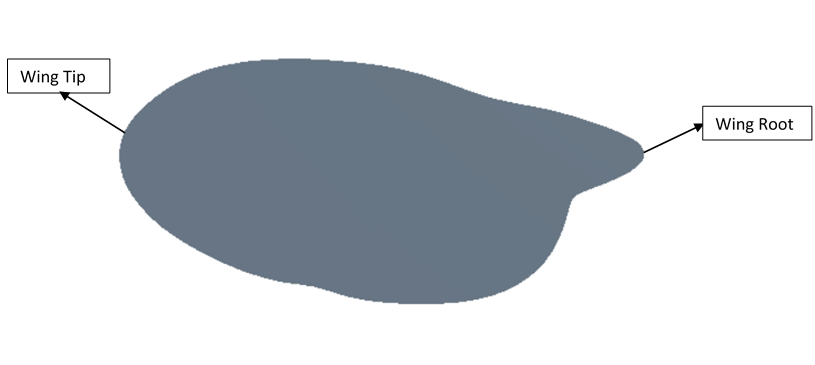
\includegraphics[width=0.8\textwidth]{include/wing.png}
  \captionsetup{justification=centering}
  \caption{Fruit fly wing geometry}
  \label{fig:your_label}
\end{figure}


\section{Pre-Processing}
\subsection{Geometry Preparation}
The fruit fly wing geometry used in the simulation is taken from literature\cite{kinematics1}. According to Perl et al, The wing's shape and size were determined by calculating the polygon defined by ten designated wing landmarks. These landmarks facilitated the acquisition of wing coordinates, forming the basis for the subsequent computation of wing shape and surface area. The primary components of variation in shape were defined from the landmark data. This involved employing Procrustes superimposition on the landmark data, which encompassed reflection, scaling (utilizing centroid size), and rotation. These transformations were applied to align the wings, minimizing deviations from the overall mean shape. Consequently, this systematic procedure enabled the characterization of shape variations within the wings. The CAD geometry imported to the STAR-CCM+ software is shown in Fig.3.1. The wing geometry is scaled such that the wing span measures 2.5mm. Also to ensure that the initial position of the root matches with the trajectory, the origin of the CAD geometry is defined at the root itself while importing to STAR-CCM+.


\subsection{Wing Kinematics Dataset for Simulation}
To define the wing beat motion in STAR-CCM+, a set of Euler angles and spatial coordinates of the wing root is derived from the Fourier series approximations. The wing beat frequency of 218 Hz was considered and the entire cycle time was discretized into 1000 instances. With the help of MATLAB, time series data of Euler angles and root position is generated and stored as tabulated files. The coordinates of the root in the dataset are modified such that the initial set of root coordinates corresponds to the origin of the wing which is positioned at its root. This is done by subtracting the root coordinates obtained while importing the wing to STAR-CCM+ from all the sets of root coordinates in the dataset. By doing this modification, we can ensure that the root will be positioned at the desired position from the set of root trajectory coordinates we have in the dataset.
The dataset used for specifying motion is given in the Appendix 1 section.

\subsection{Computational Domain and Grid Generation} 

\begin{figure}[H]
\centering
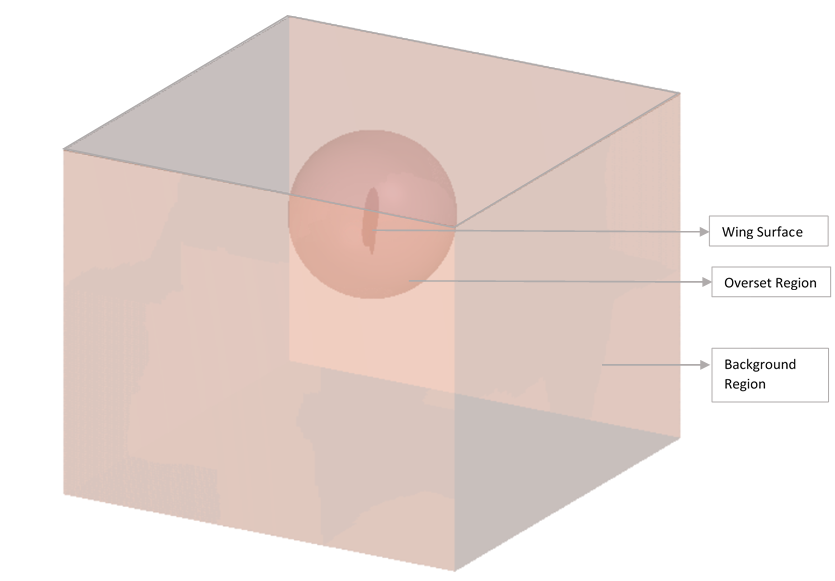
\includegraphics[width=0.8\linewidth, ]{include/Computationalregions.png}
\label{computational domain} 
\captionsetup{justification=centering}
\caption{Computational domain used in simulation}
\end{figure}
The computational domain consists of two regions namely background region and overset region and is shown in Fig.3.2. The overset region is generated by subtractive boolean operation of the wing geometry from an initial sphere part. The span of the fruit fly wing geometry considered is 2.5 mm. Accordingly, the background region is sized to be 8 times larger in dimensions to avoid any boundary influence. The overset is centered approximately at the geometric center of the wing.
Workflow followed to create the computational domain is shown in Fig.3.3.

\begin{figure}[H]
\centering
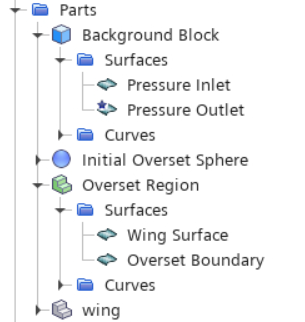
\includegraphics[width=0.4\linewidth, ]{include/domainsetup.png}
\label{computational domain setup} 
\captionsetup{justification=centering}
\caption{Steps to create computational domain}
\end{figure}

\begin{figure}[H]
\centering
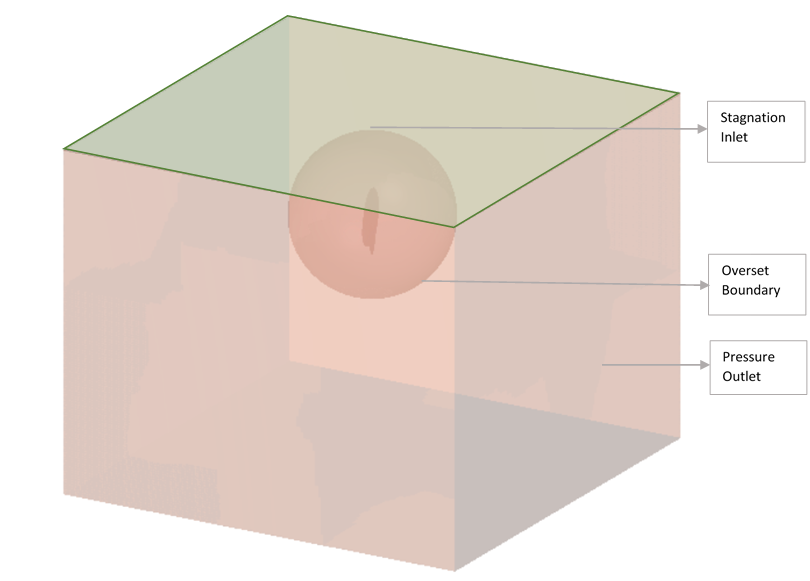
\includegraphics[width=0.8\linewidth, ]{include/regionboundaries.png}
\label{computational domain setup} 
\captionsetup{justification=centering}
\caption{Boundary conditions used at various region boundaries}
\end{figure}

From the computational domain, regions and corresponding boundaries are created. Stagnation inlet boundary condition is used to define the top boundary of the background region. Since we are simulating the hovering phase of flight, stagnation inlet condition is used to specify zero velocity at the top boundary and atmospheric pressure. The other boundaries of the background region are defined using pressure outlet conditions. The overset region is defined as the overset mesh type and the boundary between the overset region and the background region is created as an overset boundary. The overset boundary is later used to define the overset mesh interface. 
The different boundary conditions used at various boundaries of the two regions are shown in Fig.3.4.

\begin{figure}[H]
\centering
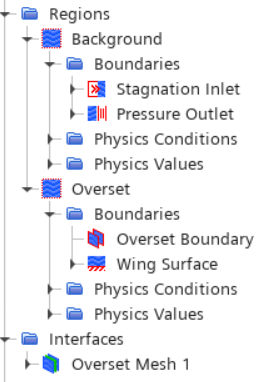
\includegraphics[width=0.4\linewidth, ]{include/regbndry.png}
\label{computational domain setup} 
\captionsetup{justification=centering}
\caption{Steps to setting up boundary conditions}
\end{figure}

A grid independence study was not done for this work. The mesh settings are taken from experience. And the computational resources permitted us to generate and use a uniform fine mesh. The base size for the background regions was set as 0.1 mm. The target size for the overset boundary was also kept at 0.1 mm in size. The minimum surface size for the overset region used is 0.005 mm and a very slow volumetric growth rate was chosen inside the overset region. 
\begin{figure}[H]
\centering
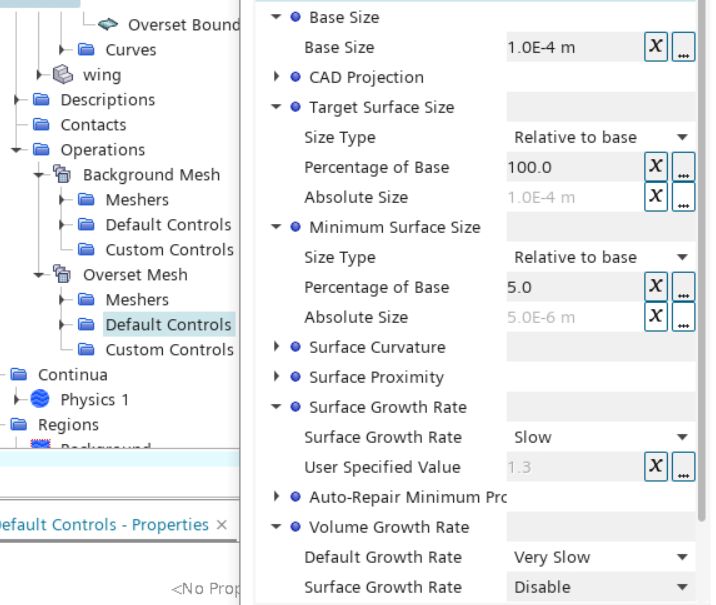
\includegraphics[width=0.6\linewidth, ]{include/oversetmeshcontrol.png}
\label{oversetmesh}
\captionsetup{justification=centering}
\caption{Mesh control for overset mesh}
\end{figure}
The overset mesh has to replace the mesh region of the background at each time step since the overset is in motion. The entire mesh cannot be updated each time as it is computationally expensive and time-consuming. To overcome this alternate hole cutting region is defined to the overset mesh. This makes the overlapped mesh region from the background be removed from computation during the motion. This necessitates the mesh size to be uniform and of similar order at the interface between the overset and background. Adaptive Mesh Refinement (AMR) setting is used to smoothen the interface between overset and background during each time step. The default controls used to set up the overset mesh are shown in Fig.3.6. The generated computational grid is shown in Fig.3.7. A section view showing the overset region is shown in Fig3.8.

\begin{figure}[H]
\centering
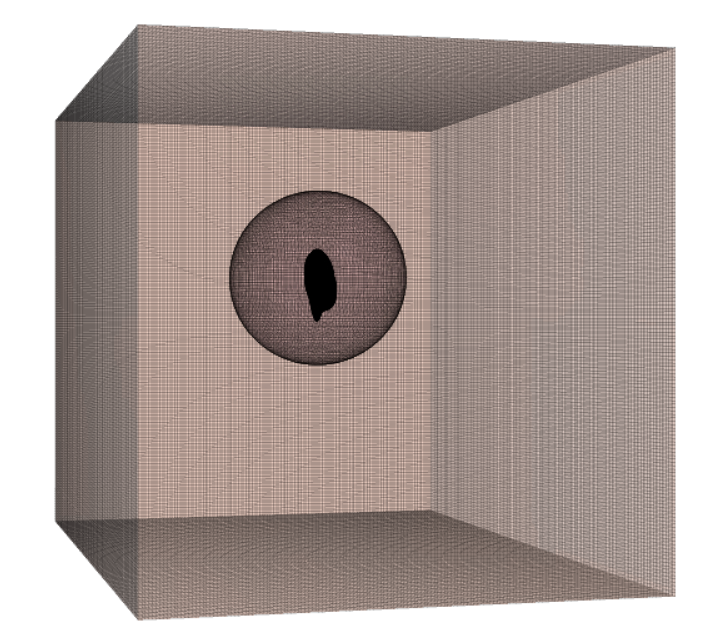
\includegraphics[width=0.55\linewidth, ]{include/Mesh.png}
\label{grid} 
\captionsetup{justification=centering}
\caption{Computational grid}
\end{figure}

\begin{figure}[H]
\centering
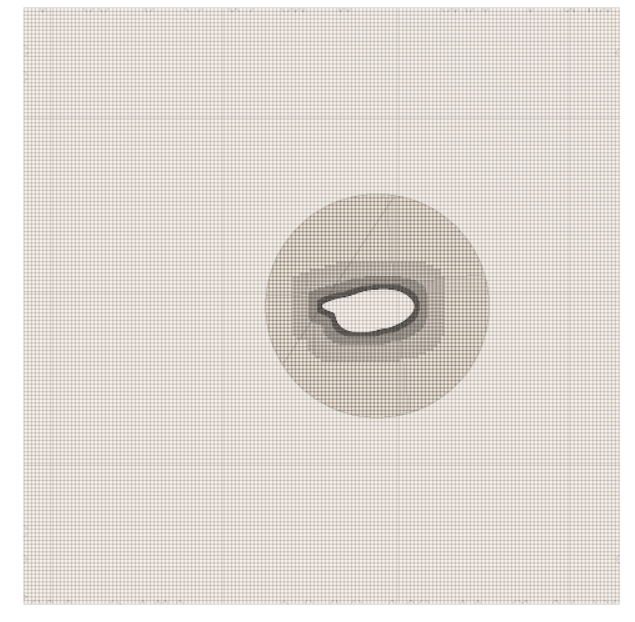
\includegraphics[width=0.5\linewidth, ]{include/sectionmesh.png}
\label{gridsection} 
\captionsetup{justification=centering}
\caption{Computational grid section view}
\end{figure}

\subsection{Setting Up Wing Beat Motion in STAR-CCM+}
In order to define the motion of the wing relevant coordinate systems are defined initially. The root trajectory of the wing is defined with respect to the laboratory coordinate system. In order to establish translation of the wing root along the defined trajectory, a coordinate system named $Trajectory$ is used. Further to specify the Euler angles rotating local coordinate systems are defined to the translating $Trajectory$ coordinate system. The image showing the Laboratory coordinate system and translating $Trajectory$ coordinate system positioned at the wing root along with the highlighted root trajectory is shown in Fig 3.9.

\begin{figure}[H]
  \centering
  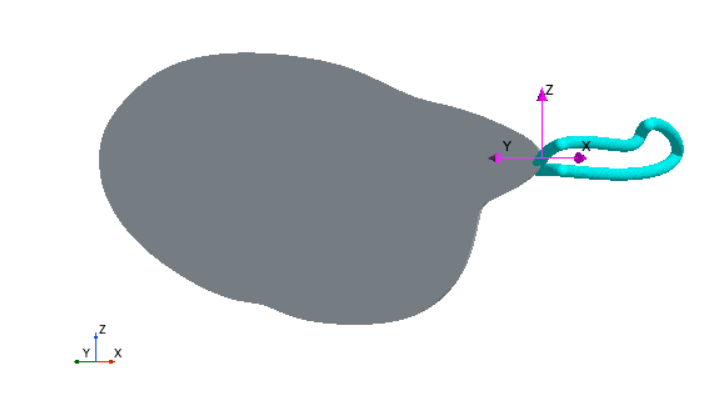
\includegraphics[width=0.8\textwidth]{include/Trajectory.png}
  \captionsetup{justification=centering}
  \caption{Laboratory and translating root-based Trajectory coordinate systems}
  \label{fig:your_label}
\end{figure}

The local coordinate systems to $Trajectory$ are named $Yaw$,$Pitch$ and $Roll$. The stroke angle is defined with respect to the $Yaw$ coordinate system. The pitch angle is defined with respect to the $Pitch$ coordinate system and the elevation angle with respect to the $Roll$ coordinate system. The tree showing the different coordinate systems used is shown in Fig 3.10. The superimposed rotational coordinate systems are shown in Fig 3.11.

\begin{figure}[H]
  \centering
  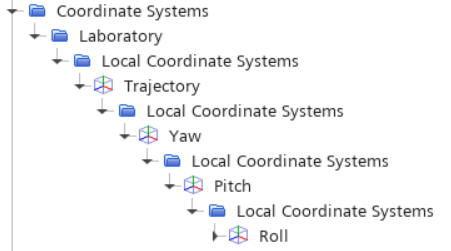
\includegraphics[width=0.6\textwidth]{include/Coordinatesystems.png}
  \captionsetup{justification=centering}
  \caption{Coordinate systems used to define motion}
  \label{fig:your_label}
\end{figure}

\begin{figure}[H]
  \centering
  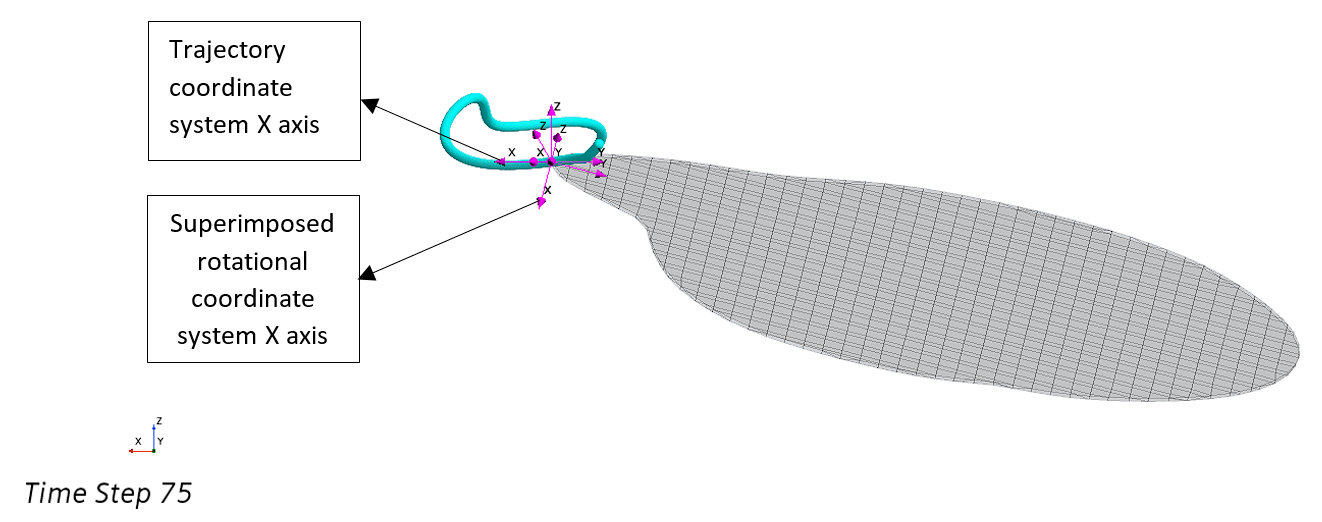
\includegraphics[width=0.9\textwidth]{include/superimposed.png}
  \captionsetup{justification=centering}
  \caption{Superimposed coordinate systems used to rotational motions}
  \label{fig:your_label}
\end{figure}

\begin{figure}[H]
  \centering
  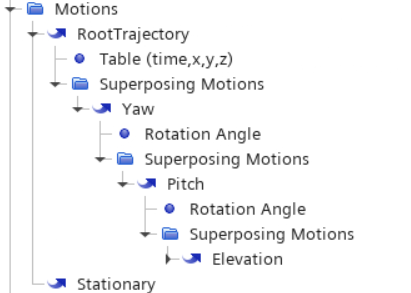
\includegraphics[width=0.6\textwidth]{include/motions.png}
  \captionsetup{justification=centering}
  \caption{Define translation and superimposing rotations}
  \label{fig:your_label}
\end{figure}


\begin{figure}[H]
  \centering
  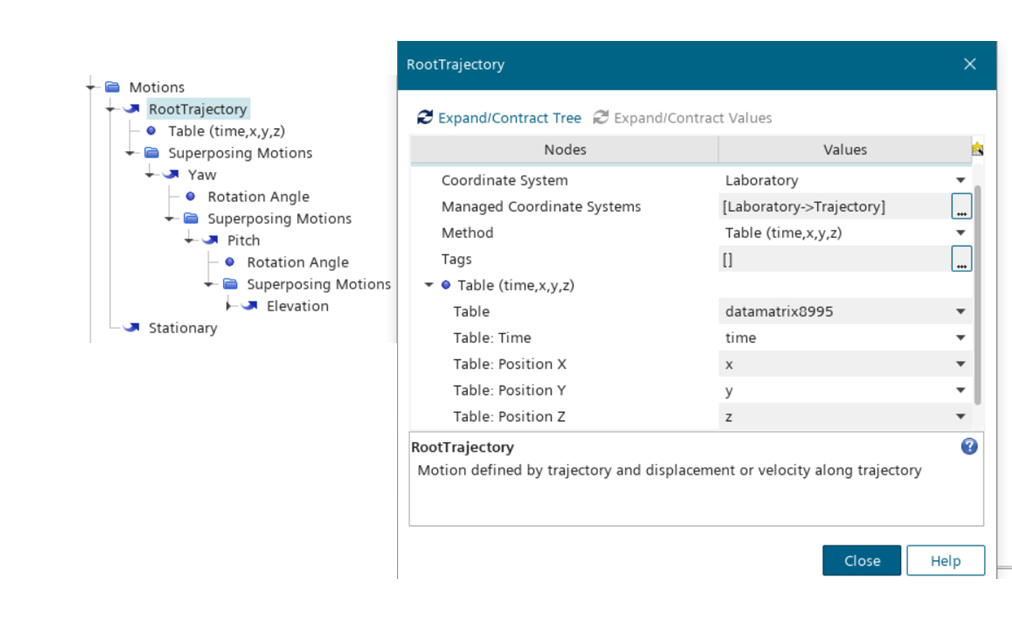
\includegraphics[width=0.8
  \textwidth]{include/translationspec.png}
  \captionsetup{justification=centering}
  \caption{Root translation parameters}
  \label{fig:your_label}
\end{figure}

Using the different coordinate systems translation and rotations of the wing are defined. The combined translation and rotation motion is then assigned to the overset region. The positional and Euler angle data from the dataset is plugged into corresponding coordinate systems.
This step is achieved using the $Motions$ node in STAR-CCM+. The procedure for specifying the motion to the overset region is shown step by step in figures Fig 3.12, Fig 3.13, Fig 3.14.
\\
\\
While defining the translation to the trajectory as in steps from Fig.3.13, The motion is managed by a $Trajectory$ coordinate system whose translation position along the trajectory is defined with respect to the global $Laboratory$ coordinate system. The root coordinates are plugged in as a time position table. In a similar fashion, the superimposed rotations are also defined. Fig.3.14 shows the parameters set for this.


\begin{figure}
  \centering
  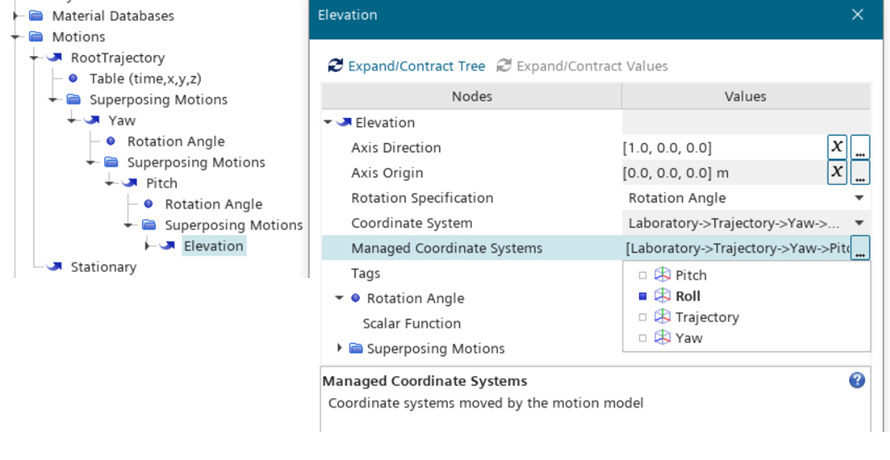
\includegraphics[width=0.8
  \textwidth]{include/elevationset.png}
  \captionsetup{justification=centering}
  \caption{Superimposed motion parameters}
  \label{fig:your_label}
\end{figure}

\begin{figure}[H]
  \centering
  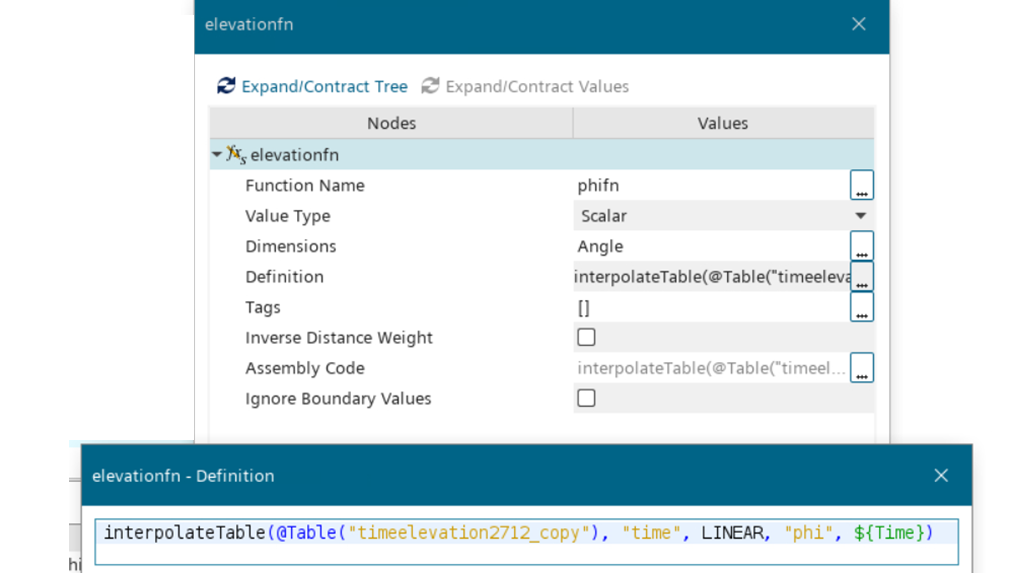
\includegraphics[width=0.8
  \textwidth]{include/elevationfnn.png}
  \captionsetup{justification=centering}
  \caption{Rotation angle scalar function}
  \label{fig:your_label}
\end{figure}


The axis of rotation corresponding to the local coordinate system is set. Also, the motion is managed by the respective local coordinate system. In the case of the elevation motion, The reference coordinate system is the $Pitch$ coordinate system, and the managed coordinate system is the $Roll$ coordinate system. The rotation angle is given as a scalar function of time. The scalar function is defined in the $Field functions$ node using the time series table for elevation angle. The syntax used to define the interpolation scalar function named $elevationfn$ is given in Fig 3.15. The pitch and yaw motions are defined similarly. Once the motions are defined they are assigned to the overset region in its $motion\_specification$. This is shown in Fig 3.16.
\begin{figure}[H]
  \centering
  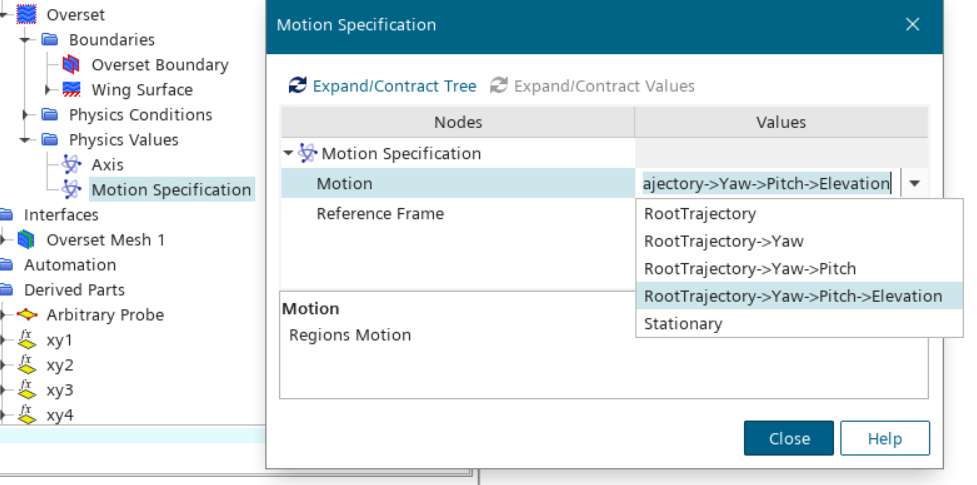
\includegraphics[width=0.8
  \textwidth]{include/motion specification.png}
  \captionsetup{justification=centering}
  \caption{Motion specification to overset region}
  \label{fig:your_label}
\end{figure}

\newline
\new
\section{Physics and Solver Setup}


Since the observed Reynolds number with the flow field surrounding the fruit fly wing is low and magnitudes near 100, An incompressible flow field is assumed. The k-omega turbulence model is enabled for better resolution of flow separation effects. The implicit unsteady solver with a time step equal to $4.58\mu s$ is also used. This time step corresponds to 1/1000 of the cycle time for fruit fly wing beat. Further as mentioned before, Adaptive mesh refinement is used to carry out overset mesh interface refinement. The physics setup for the simulation is shown in Fig 3.17.
The simulation was done for 8 wing beat cycles using a cluster computing platform. 

\begin{figure}[H]
  \centering
  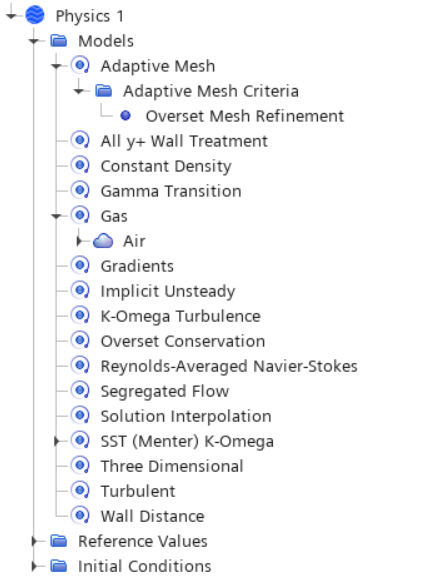
\includegraphics[width=0.6
  \textwidth]{include/physiscs.png}
  \captionsetup{justification=centering}
  \caption{Physics setup}
  \label{fig:your_label}
\end{figure}

\section{Post-Processing}

To study the passiveness of pitch and stroke motions, we were particularly interested in recording the variation of the wing's pitching moment with respect to pitch angle as well as the variation of stroke moment with respect to stroke angle for each time-step. For this monitors of pitching moment and stroke moment are added to post-process. Also, the lift and drag characteristics of the wing over the cycle are also plotted. Velocity contours of the flow field are also captured as scenes. From the monitored data finally, hysteresis plots for pitch and stroke motions were generated for analysis.
\\
\\
The workflow followed in the work for carrying out the CFD simulation is based on Simcenter STAR-CCM+ documentation:\\ 
$Trajectory\_Motion - Paint\_Dipping\_of\_a\_Chassis\_on\_a\_Fixed\_Skid$



















